% -- Approach ---------------------------------------

\section{Approach}

Our extracted kernel can be found in appendix \ref{sec:satd}. In order to make the extracted kernel qualified for compilation and execution, a few things have to be altered. First, the new file has to be recognized by the \mcode{makefile} in the rovex-examples directory. By executing \mcode{make byte-} command two files are created:
\begin{itemize}
	\item \mcode{bytecode}, containing all the intstructions to be executed by the $\rho$-VEX
	\item \mcode{bytedata}, containing the pixels of the input stream
\end{itemize}

Second, some type definitions have to be made. Originally, \mcode{pixel\_satd\_8x4} resides in the \mcode{pixel.c} file of the x264 application. When extracting this kernel, all prior knowledge is lost and has to be defined again. Then, in order to make the kernel compile and run on the $\rho$-VEX, the development board has to be reset and started. \mcode{Bytecode} has to be written to the instruction memory (\mcode{rex-imemory}) and \mcode{bytedata} to the data memory (\mcode{rvex-dmemory}). Finally, the calculated result should be returned to the host. Figure X shows the $\rho$-VEX memory layout for our kernel.

\subsection{Adjusting the \mcode{makefile}}

In order to make the makefile recognize the extracted kernel, the file can simply be added to the \mcode{EXECUTABLES}. Other files are already in the \mcode{makefile} (e.g. \mcode{adpcm}), but these can be removed since we will not need them for our application. An important issue is the difference between logical memory and physical memory. While the first address of a logical memory is obviously zero, the physical memory can have the first part of the register being occupied by the operating system. For the $\rho$-VEX, the first address which is allowed to be (over)written is 120. Thus, when writing for example the result of the kernel to the logical address '0', it actually should be written to the physical address '120' of the data memory. This can be done using \mcode{\_\_DATA\_START} to indicate the start address.

Despite the fact that this is a rather simplistic operation, it took us some struggling to have this action confirmed as correct. For example, we were told to remove the \mcode{AUTOINLINE} flag which resulted in a lot of wrong hexdumps. Also, half way the lab a fix has been made to eliminate the issue of the logical and physical addresses. All references to \mcode{\_\_DATA\_START} had to be removed again, which felt like we had wasted lots of time. Unfortunately, we still had major problems getting the application to run correctly. As it turned out, the fix had only affected the 'home' directory. In order to avoid conflicting files, we had created a separate folder named 'lab2' from where we executed the application. Due to this, the fix did not reach our code and thus did not eliminate the start address issue.

\subsection{Type Definition}

As stated earlier, an extracted kernel is unable to obtain information from previous code. Consequently, all parameters have to be pre-defined. Table \ref{typedef} shows all required type definitions.

% -- Type Definitions ---------------------------------------
\begin{table}[htb]%
\begin{tabular}{lll}
	\bf{Parameter} 					& \bf{Type definition} 					& \bf{Motivation}\\ \cline{1-3}
	\mcode{intptr\_t}				&	\mcode{unsigned int}					& This parameter represents the stride, which cannot be $<$0\\
	\mcode{pixel}						& \mcode{unsigned char}					&	Pixels are made out of bytes, which have 8 bits (like a \mcode{char})\\
	\mcode{sum\_t}					&	\mcode{short int}							& Same type definition as in the source code (16 bits)\\
	\mcode{sum2\_t}					& \mcode{long int}							& Same type definition as in the source code (32 bits)\\
	\mcode{BIT\_DEPTH}			& defined as 8									& Also in the source code, plus the kernel handles pixels (bytes)\\
	\mcode{BIT\_PER\_SUM}		&	(8 * \mcode{sizeof(sum\_t)})	& Also predefined as in the source code, being 8 as well\\
\end{tabular}
\caption{Type definitions in the extracted kernel file.}
\label{typedef}
\end{table}

\subsection{Communication between the MicroBlaze and the $\rho$-VEX}

In order to delegate the \mcode{satd\_8x4} kernel from the MicroBlaze to the $\rho$-VEX, both the environments need to communicate with each other. When executing the \mcode{x264} application, the MicroBlaze has to load the instructions of the extracted kernel into the instruction memory of the $\rho$-VEX and the data (for which the SATD has to be evaluated) into the data memory. This is when the source code of \mcode{x264} becomes involved. The \mcode{pixel\_satd\_8x4 kernel}, which is residing in the \mcode{pixel.c} file of the application, needs to be overwritten. Instead of calculating the SATD, it should send the instructions and input to the $\rho$-VEX. The commands \ref{eq:imem} and \ref{eq:dmem} are therefore added to the \mcode{pixel.c} file of the \mcode{x264} application. These pixels are written at physical address 120, the first address on the $\rho$-VEX that is not set apart for communication between the driver and the $\rho$-VEX. Also, an empty pixel is written after \mcode{bytedata} in order to make space for writing the result. 

\begin{figure}
	\centering
	\begin{subfigure} [h] {0.3\textwidth}
		\centering
		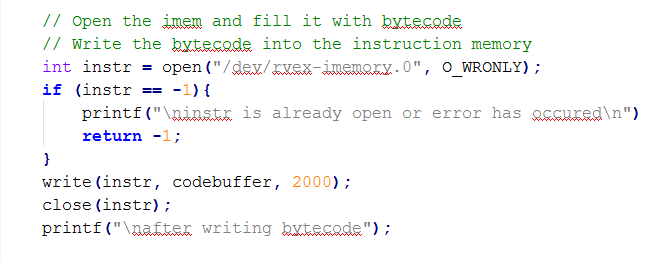
\includegraphics[width=150px]{Pictures/imem}
		\caption{Bytecode}
		\label{fig:imem}
	\end{subfigure}
	\quad
	\begin{subfigure} [h] {0.3\textwidth}
		\centering
		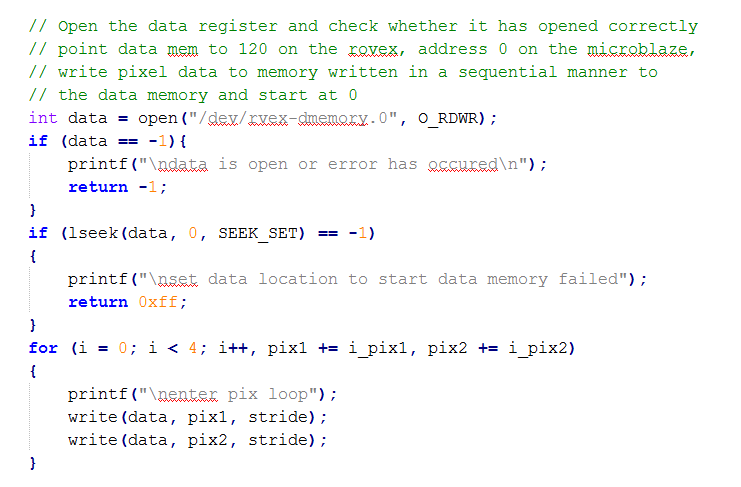
\includegraphics[width=150px]{Pictures/dmem}
		\caption{Bytedata}
		\label{fig:dmem}
	\end{subfigure}
	\quad
	\begin{subfigure} [h] {0.3\textwidth}
		\centering
		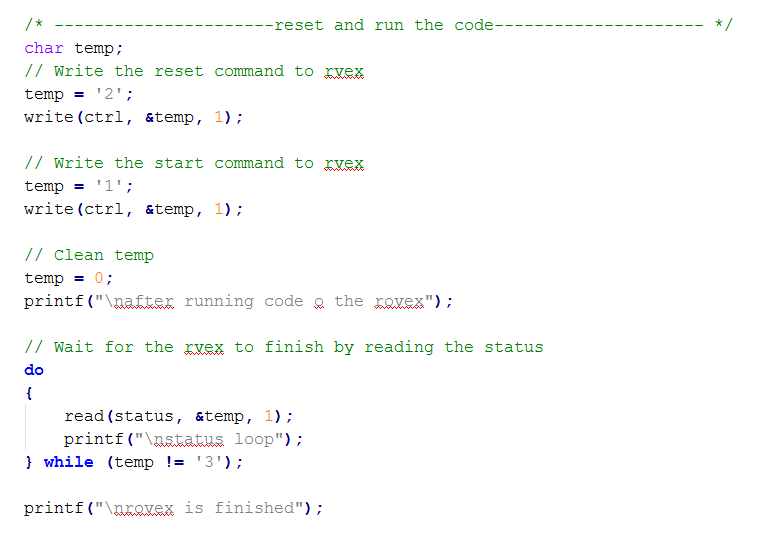
\includegraphics[width=150px]{Pictures/smem}
		\caption{Reset, set and get the status of the $\rho$-VEX}
		\label{fig:smem}
	\end{subfigure}
	\quad
\caption{Commands for reading from and writing to the $\rho$-VEX}%
\label{}%
\end{figure}

To control the $\rho$-VEX from the x264 application, the control memory should also be written. By first setting the control to \mcode{'2'}, the $\rho$-VEX is being reset. It can then be started by writing \mcode{'1'} to control, telling the $\rho$-VEX to start calculating the satd of the two pixels. While calculating, the status of the $\rho$-VEX can be checked in a \mcode{while}-loop by reading the status variable of the status memory (\mcode{rvex-smemory}). When the \mcode{satd} kernel is finished, the result can be read from the data memory. See also \ref{fig:smem}.

\subsection{Result Hyphothesis}

By having the computational intensive kernel being run concurrently on a co-processor, one could expect an overal speedup of the application. A problem is, however, that the \mcode{bytecode} and \mcode{bytedata} have to be sent to the $\rho$-VEX every time the kernel is being called. \mcode{Bytedata} contains two new pixels of which the SATD has to be calculated, \mcode{bytecode} the kernel instructions. Because of this constant data traffic between the MicroBlaze and the $\rho$-VEX we don't think the intended speed up is achieved.


The reason that \mcode{bytecode} has to be sent every time the kernel is called, is that the three FPGAs are shared among a lot of students. When running their application concurrently, the instruction memory is constantly overwritten by another group. If there was a one-to-one setup, \mcode{bytecode} could have to been placed in \mcode{main.c}, written tot the \mcode{imemory} of the $\rho$-VEX once when starting the application. 


